\section{Application to protoplanetary disks}\label{application} 
As an application of our linear models, we estimate where in a
protoplanetary disk do the thermodynamic conditions allow the VSI to
operate. For a realistic disk one can consider the energy equation
with radiative cooling, 
\begin{align}\label{real_energy}
  % \rho T \frac{DS}{Dt} = - \left(\nabla\cdot\bm{F} - Q_+\right), 
  \frac{\p P}{\p t} + \bm{v}\cdot\nabla P +\gamma P \nabla\cdot\bm{v} = - \frac{P}{\rho T
    c_v}\left(\nabla\cdot\bm{F} - Q_+\right), 
\end{align}
where $c_v$ is the heat capacity at constant
volume, 
$\bm{F}$ is the radiative flux and $Q_+$ is a heating
term to permit an equilibrium solution. 

One should now model in detail each of the terms on the RHS of
Eq. \ref{real_energy}, linearize them, then solve 
the resulting linear eigenvalue problem. This is beyond 
the scope of the present work. Here, we take the simpler approach of
modeling the linearized RHS of Eq. \ref{real_energy} such that it can 
be represented by a thermal relaxation time $t_c$. 
To do so, we first consider separately perturbations
with radial lengthscales $l\gg l_\mathrm{rad}$ and  
$l\ll l_\mathrm{rad}$, where      
\begin{align}\label{lrad}
  l_\mathrm{rad} \equiv \frac{1}{\kappa_d\rho} 
\end{align} 
is the photon mean-free-path and $\kappa_d$ is the (dust) opacity. 

\subsection{Radiative diffusion}
For perturbations with lengthscales $l\gg
l_\mathrm{rad}$, we assume temperature fluctuations are smoothed out
by radiative diffusion and model this in linear theory by writing the
linearized RHS of Eq. \ref{real_energy} as 
% we choose the heating term such that
% \begin{align}
%   Q_+ - \nabla\cdot\bm{F} \equiv \nabla\cdot\left[k_\mathrm{rad}\nabla
%     \left(T-T_{t=0}\right)\right], 
% \end{align} 
% where $k_\mathrm{rad}$ is the conduction coefficient to be defined
% implicitly. Eq. \ref{real_energy} becomes
% \begin{align}
%   \frac{DP}{Dt} = -\gamma P \nabla\cdot\bm{v} + \frac{P}{\rho T
%   c_v}\nabla\cdot\left[k_\mathrm{rad}\nabla\left(T-T_{t=0}\right)\right].     
% \end{align}
% When linearized, the last term on the RHS becomes
\begin{align}\label{diff_cool_proper}
  \frac{P}{\rho T c_v} \nabla\cdot\left(k_\mathrm{rad}\nabla\delta
    T\right),  
\end{align}
where $k_\mathrm{rad}$ is the conduction coefficient to be defined
implicitly. 

However, Eq. \ref{diff_cool_proper} fundamentally changes the linear
problem by introducing higher order derivatives. We defer a proper
analysis of this problem to a follow-up study. Here, we are interested
in order-of-magnitude estimates for perturbations with radial
lengthscales much smaller than vertical lengthscales. We thus proceed 
by assuming vertical derivatives can be neglected in 
Eq. \ref{diff_cool_proper} and write  
\begin{align}\label{diff_cool_approx}
  \frac{P}{\rho T c_v} \nabla\cdot\left(k_\mathrm{rad}\nabla\delta
    T\right) &\to -\frac{k_\mathrm{rad}}{\rho
    c_v}k_x^2P\left(\frac{\delta T}{T}\right)\notag\\
  &\equiv -\eta k_x^2 \left(\delta P - \frac{P}{\rho}\delta\rho\right), 
\end{align}
% we are interested in radially-thin perturbations  
where $\eta=k_\mathrm{rad}/\rho c_v$ is the diffusion coefficient and
is given in terms of physical disk parameters as 
\begin{align}\label{eta_def}
  \eta = \frac{16\sigma_s T^3}{3\kappa_d\rho^2 c_v}, 
\end{align}
where $\sigma_s$ is the Stefan-Boltzmann constant. 
From Eq. \ref{diff_cool_approx} we identify the scale-dependent thermal relaxation
time for diffusion as 
\begin{align}\label{tc_diff_cool} 
  t_\mathrm{diff} = \frac{1}{\eta k_x^2}.%\equiv \frac{\Omega_k^{-1}}{\hat{\eta}\khat^2}, 
\end{align}
% where $\hat{\eta} = \eta/H^2\Omega_k$ is the 
% dimensionless diffusion coefficient. 


\subsection{Newtonian cooling}\label{newton_cool}
For perturbations with small lengthscales, $l\ll l_\mathrm{rad}$, 
the disk is optically thin. In this case, we assume 
Newtonian cooling can be applied, which is the thermal
relaxation model as adopted in our linear models. That is, temperature
flucations $\delta T$ decay on a timescale $t_\mathrm{cool}$,
independent of $k_x$. For simplicity, we take  
\begin{align}
  t_\mathrm{cool} = \frac{l_\mathrm{rad}^2}{3\eta}. 
\end{align}
We note that $t_\mathrm{cool}$ does not explicitly depend on $\rho$. 

\subsection{A model for combined thermal relaxation}\label{toy_relax}
To unify $t_\mathrm{cool}$ and $t_\mathrm{diff}$, we define the
effective thermal relaxation timescale in linear theory as
\begin{align}\label{tc_def}
  t_c &\equiv t_\mathrm{cool} + t _\mathrm{diff}. %=
  % \frac{l_\mathrm{rad}^2}{3\eta} + \frac{1}{\eta k_x^2},  
\end{align}
Eq. \ref{tc_def} is a simple prescription so
that for small scales (large $k_x$), $t_c\to t_\mathrm{cool}$, while
for large scales (small $k_x$), $t_c\to t_\mathrm{diff}$. Writing the
volume density $\rho = \Sigma\hat{\rho}/\sqrt{2\pi}H$, where
$\hat{\rho} = \rho/\rho_0$ and $\Sigma$ is the surface density at the
radius of interest, the dimensionless thermal
relaxation time $\beta$ becomes 
\begin{align}\label{real_beta}
  \beta(z;\khat) \equiv t_c\Omega_k =
  % \frac{1}{\hat{\eta}}\left[\frac{l_\mathrm{rad}^2}{3H^2}
  %   + \frac{\hat{\rho}^2(z)}{2\pi\khat^2}\right]  \simeq
  \frac{\Sigma^2\Omega_k}{\eta\rho^2}\left[\frac{1}{3\kappa_d^2\Sigma^2} 
    + \frac{\hat{\rho}^2(z)}{2\pi \khat^2}\right].
\end{align}
Note that $\beta$ depends on both the perturbation lengthscale $\khat$ 
and distance from the midplane. 

\subsection{Evaluation for a fiducial disk model}
We evaluate Eq. \ref{real_beta} for the protoplanetary disk model
described in \cite{chiang10} and summarized in Appendix \ref{mmsn}
(where an opacity model is also chosen). Defining $r_\mathrm{AU}\equiv 
r/\mathrm{AU}$, we find Eq. \ref{real_beta} becomes
\begin{align}\label{beta_mmsn}
  \beta(z; \khat) =
  &\frac{4.4\times10^5}{\mu(\gamma-1)}\left(\frac{\hat{\kappa}_d\hat{\Sigma}^2}{\hat{T}}\right)r_\mathrm{AU}^{-57/14}\notag\\ 
&\times\left[\frac{8.3\times10^{-9}}{\hat{\kappa}_d^2\hat{T}^4\hat{\Sigma}^2}r_\mathrm{AU}^{33/7}+\frac{\hat{\rho}^2(z)}{2\pi\khat^2}\right].         
\end{align} 
We refer to the case with $\gamma=1.4$, $\mu=2.33$ and the scalings
$\hat{\Sigma}=\hat{\kappa}_d=\hat{T}=1$ as the Minimum Mass Solar
Nebulae (MMSN) and $\beta=\beta_\mathrm{MMSN}$, 
\begin{align}\label{beta_mmsn_simp}
  \beta_\mathrm{MMSN} = 3.9\times10^{-3} r_\mathrm{AU}^{9/14}\left( 1 +
    1.9\times10^7\hat{\rho}^2r_\mathrm{AU}^{-33/7}\khat^{-2}\right). 
\end{align}
% where
% \begin{align}
%   \
% %  \frac{3.7\times10^{-3}}{\mu\left(\gamma-1\right)\hat{\kappa}_d\hat{T}^5}, 
% \end{align}
% and
% \begin{align}
%   \khat_0 = 4.4\times10^{3}\hat{\kappa}_d\hat{T}^2\hat{\Sigma}.
% \end{align}
It is instructive to compare the above thermal timescale 
with the criterion Eq. \ref{iso_vsi_cond} evaluated for the MMSN,     
\begin{align}\label{bcrit_mmsn}
  % \beta_\mathrm{crit} = \frac{1.44\times10^{-2}}{(\gamma
  % -1)}\left(\frac{\hat{T}}{\mu}\right)^{1/2}r_\mathrm{AU}^{2/7}. 
  \beta_\mathrm{crit,MMSN} = 0.024r_\mathrm{AU}^{2/7}. 
\end{align}

In Fig. \ref{mmsn_bcrit_bcool} we plot Eq. \ref{beta_mmsn}  with $\mu
=2.33$ $\gamma=1.4$, $\hat{T}=\hat{\Sigma}=1$ for opacity scales
$\hat{\kappa}_d=0.1, \,1 $ (MMSN) and $10$, at $z=0$ and $z=3H$. We
also plot Eq. \ref{bcrit_mmsn} in each panel.   

Consider first the MMSN shown in the middle panels of 
Fig. \ref{mmsn_bcrit_bcool}. The critical thermal timescale,
Eq. \ref{bcrit_mmsn}, is useful in the optically thin regime (where the
curves overlap), since in this limit $\beta$ does not depend on
height, as assumed in our analysis. We thus infer that the VSI can
operate at tens of AU in the MMSN.  

In the inner few AU of the MMSN, however, $\beta$ 
may be smaller or greater than $\beta_\mathrm{crit}$ depending on
$z$ as the disk transitions from an optically thick midplane to an
optically thin atmosphere. 
%Given a fixed $\khat$, one can have $\beta > \beta_\mathrm{crit}$ at
%the optically thick midplane, but with increasing height the disk 
%becomes optically thin and $\beta<\beta_\mathrm{crit}$. 
Our analytical criteria is not valid for variable $\beta$, and we must
turn to numerical solutions of the linear problem to determine whether
or not the VSI operates. We do this in the next section.   
 
Lowering the opacity, as shown in the top panels of
Fig. \ref{mmsn_bcrit_bcool}, shifts the curves inwards but also raises
them. In fact, lowering the opacity by an order of magnitude renders  
$\beta > \beta_\mathrm{crit}$ even away from the midplane. This is 
expected to stabilize the disk. Raising the opacity, as shown in 
the lower panels of Fig. \ref{mmsn_bcrit_bcool}, decreases the thermal
timescales, but shifts the curves outward, so the instability is
restricted to larger radii.  

%but
%given that the VSI depends on vertical shear, an effect that becomes
%important away from the disk midplane, the inner disk may still be
%able to develop the VSI, but it is likely restricted to the disk
%surface.   
%We remark that it is possible to satisfy $\beta<\beta_\mathrm{crit}$
%at small radii by choosing a sufficiently large $\khat$. However, our
%linear calculations suggest growth rates eventually decay as 
%$\khat\to\infty$. Thus, very small-scale VSI in the inner disk is
%probably unimportant.   

\begin{figure*}
  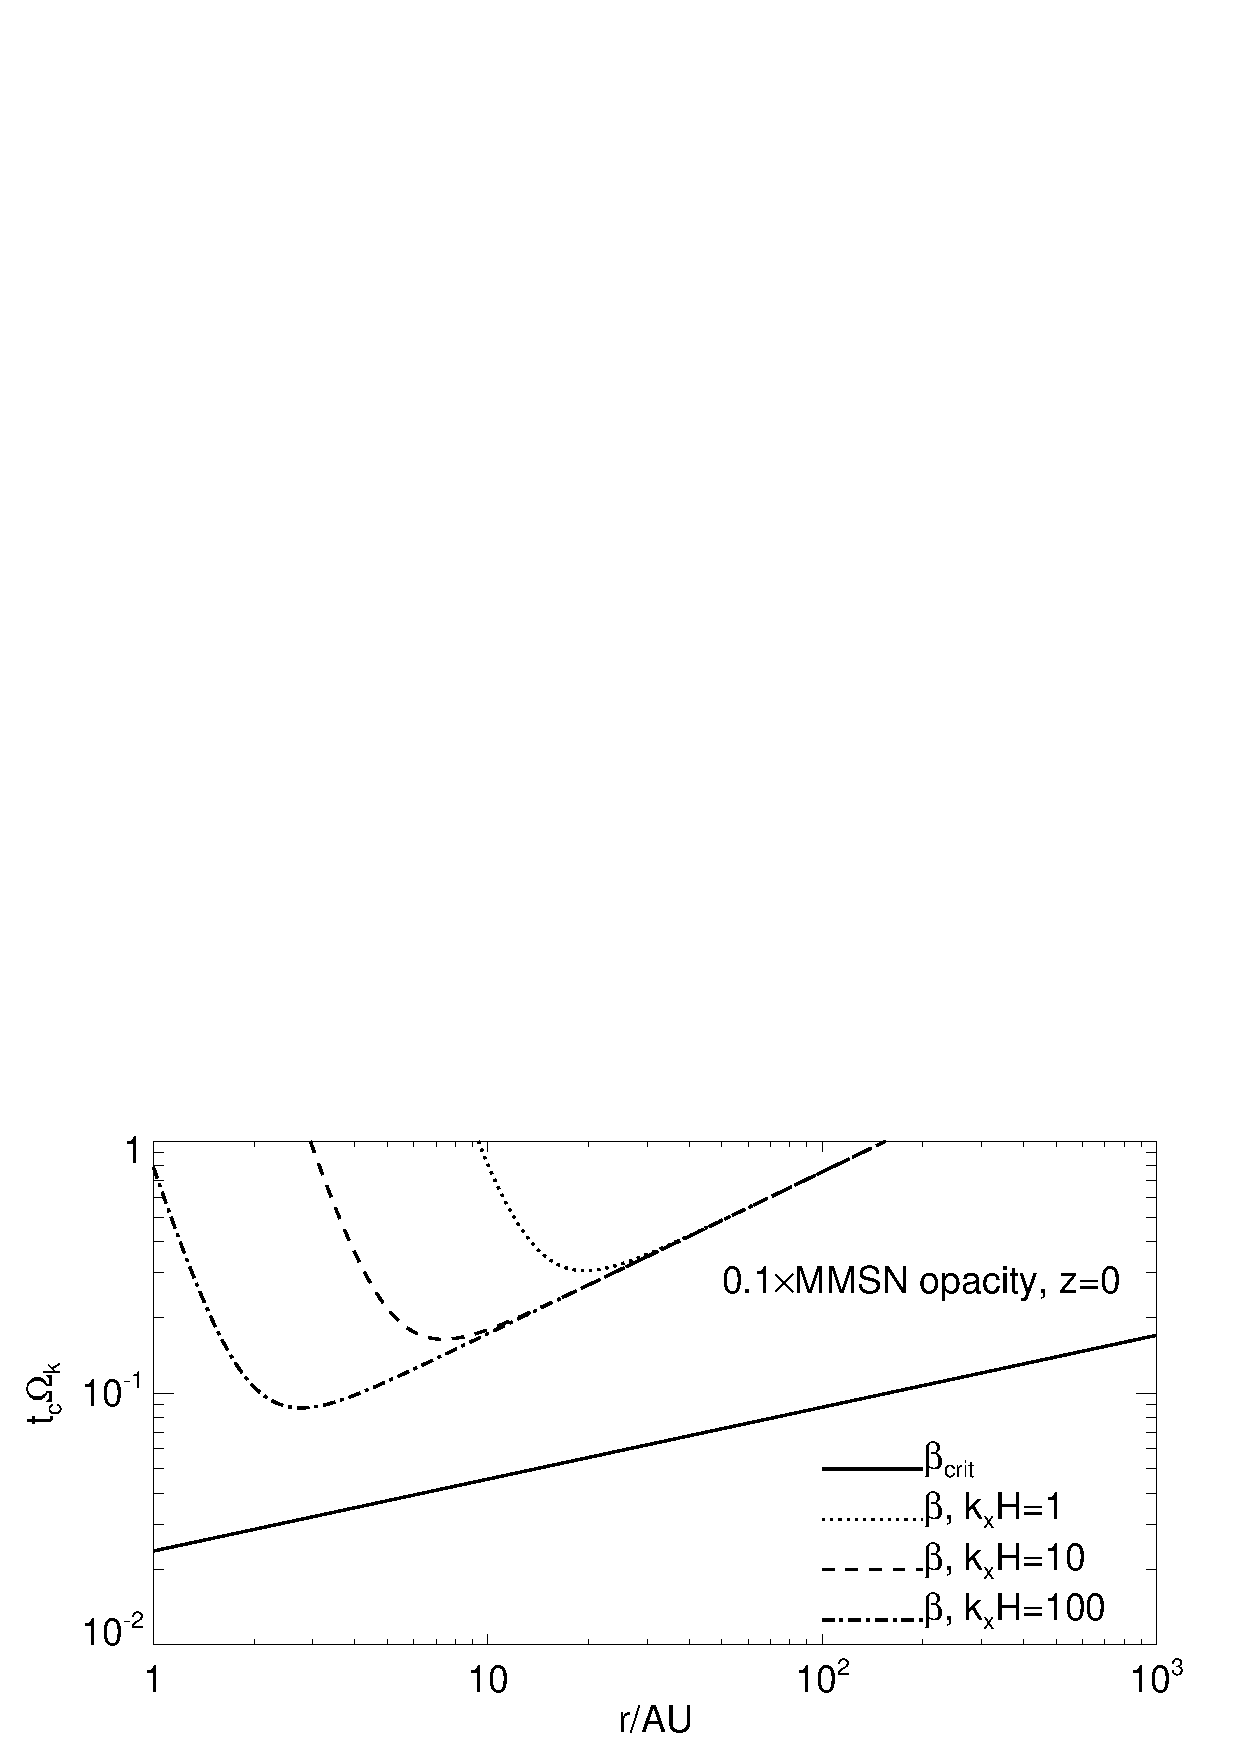
\includegraphics[scale=.47,clip=true,trim=0cm 1.8cm 0cm
  0cm]{figures/bcrit_mmsn_kap0d1_z0}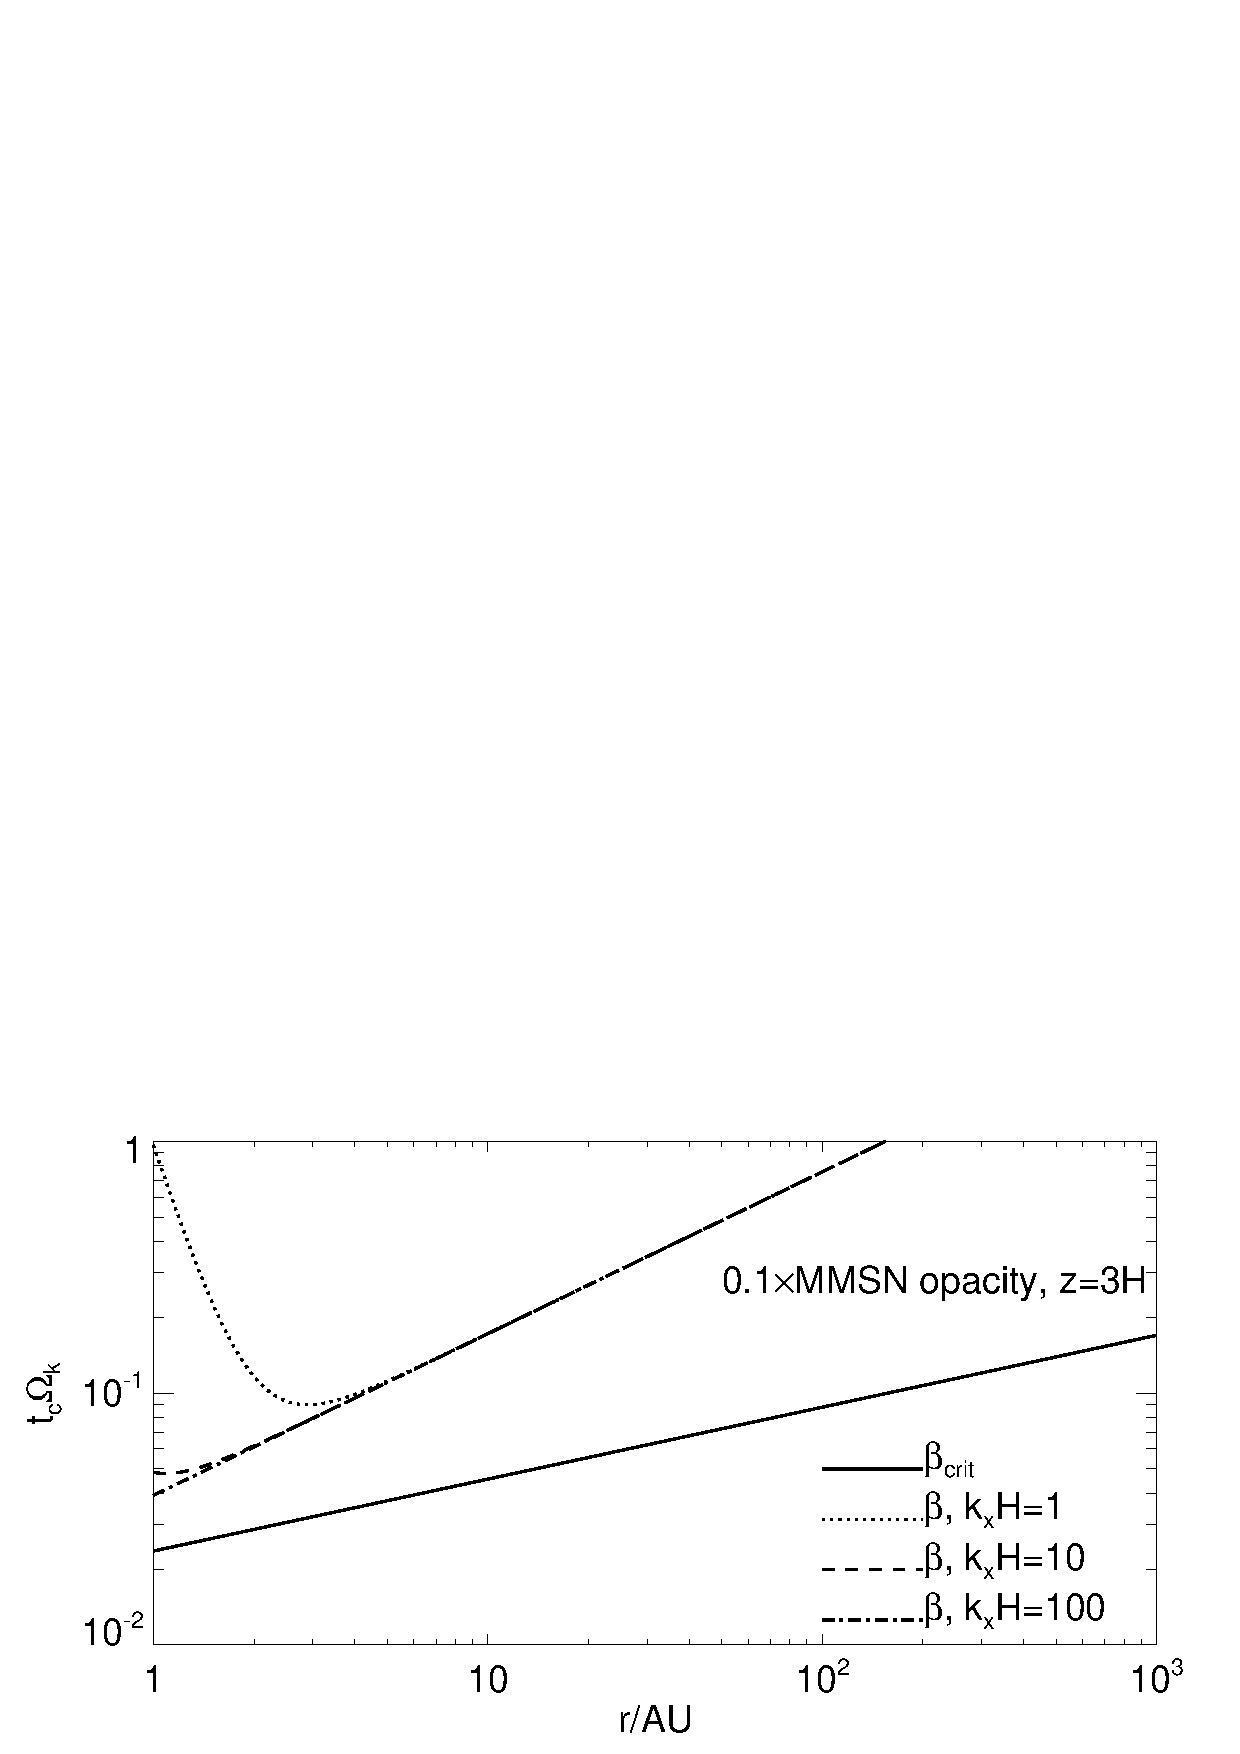
\includegraphics[scale=.47,clip=true,trim=2.5cm 1.8cm 0cm
  0cm]{figures/bcrit_mmsn_kap0d1_z3}\\ 
  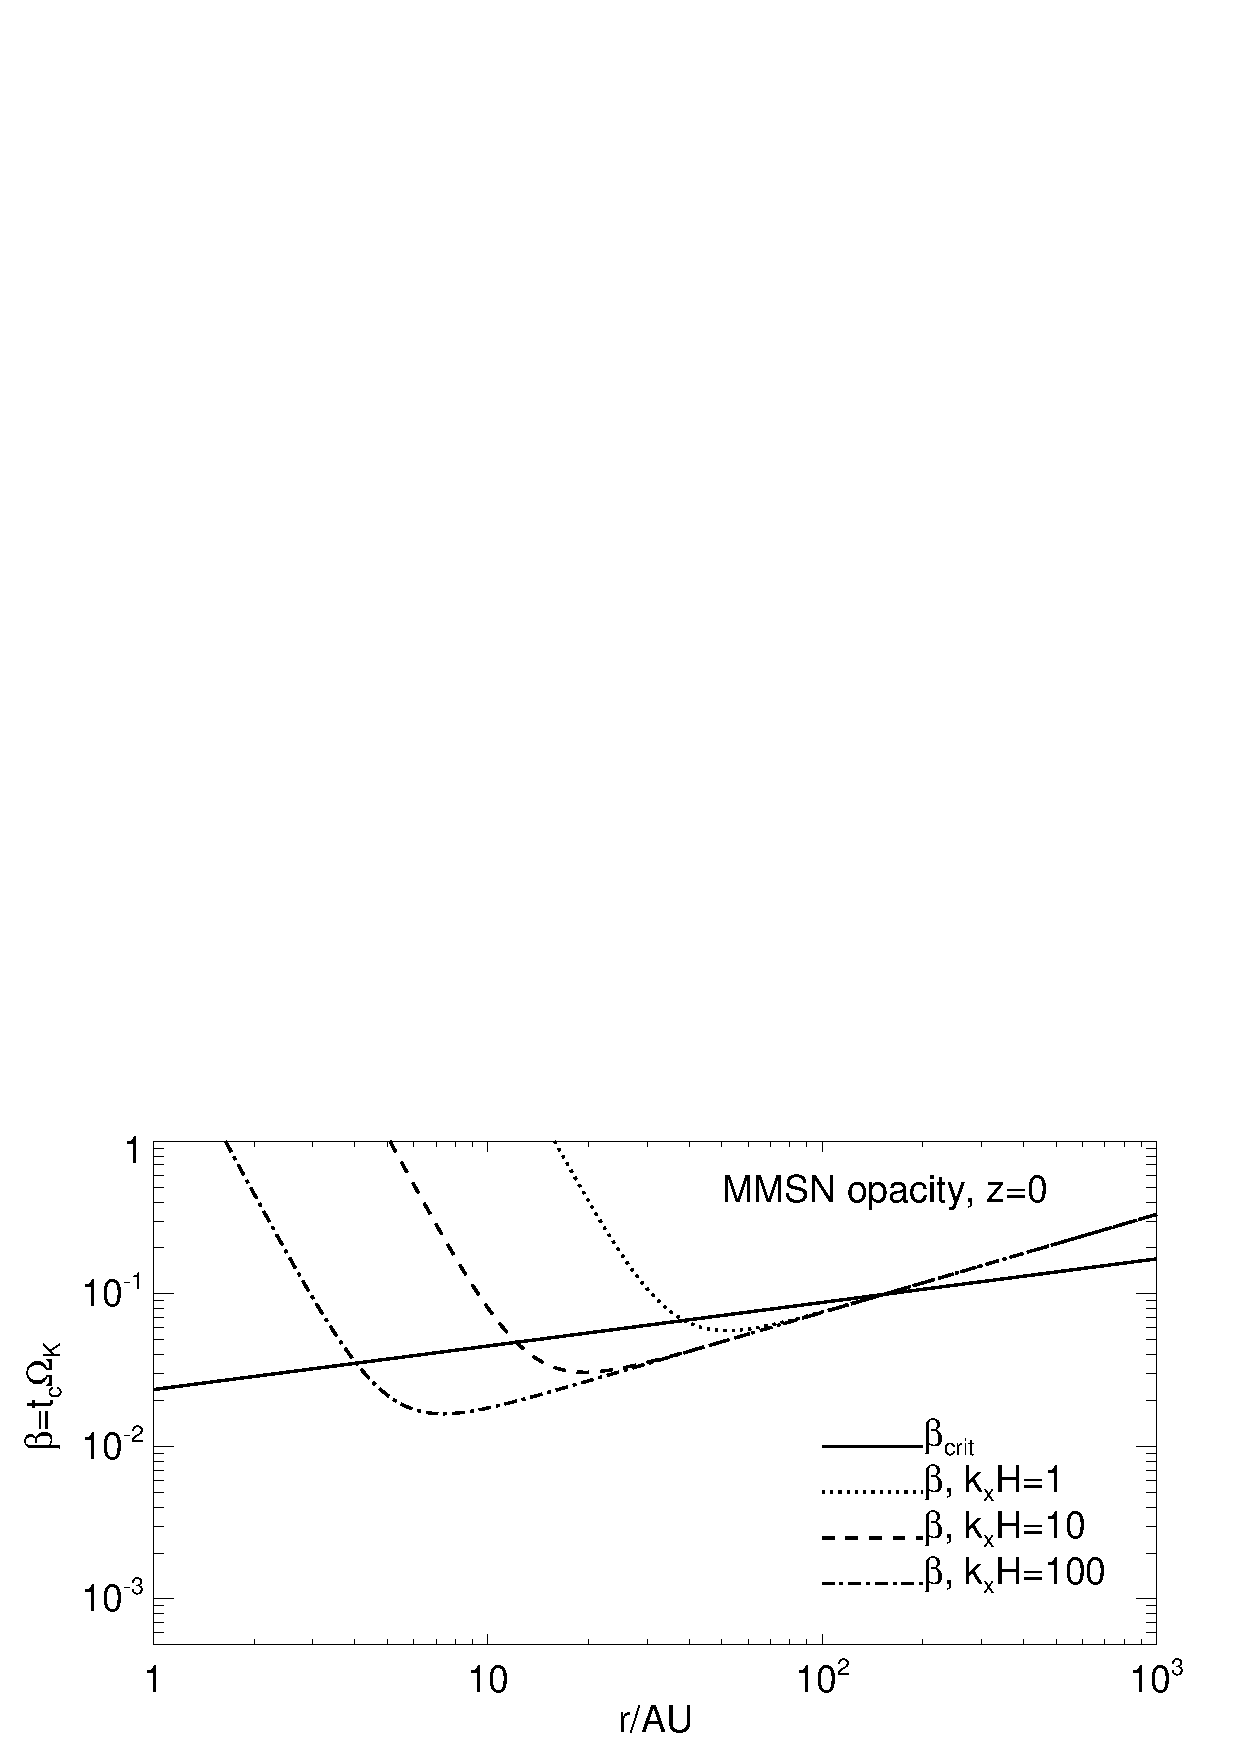
\includegraphics[scale=.47,clip=true,trim=0cm 1.8cm 0cm
  1cm]{figures/bcrit_mmsn_kap1_z0}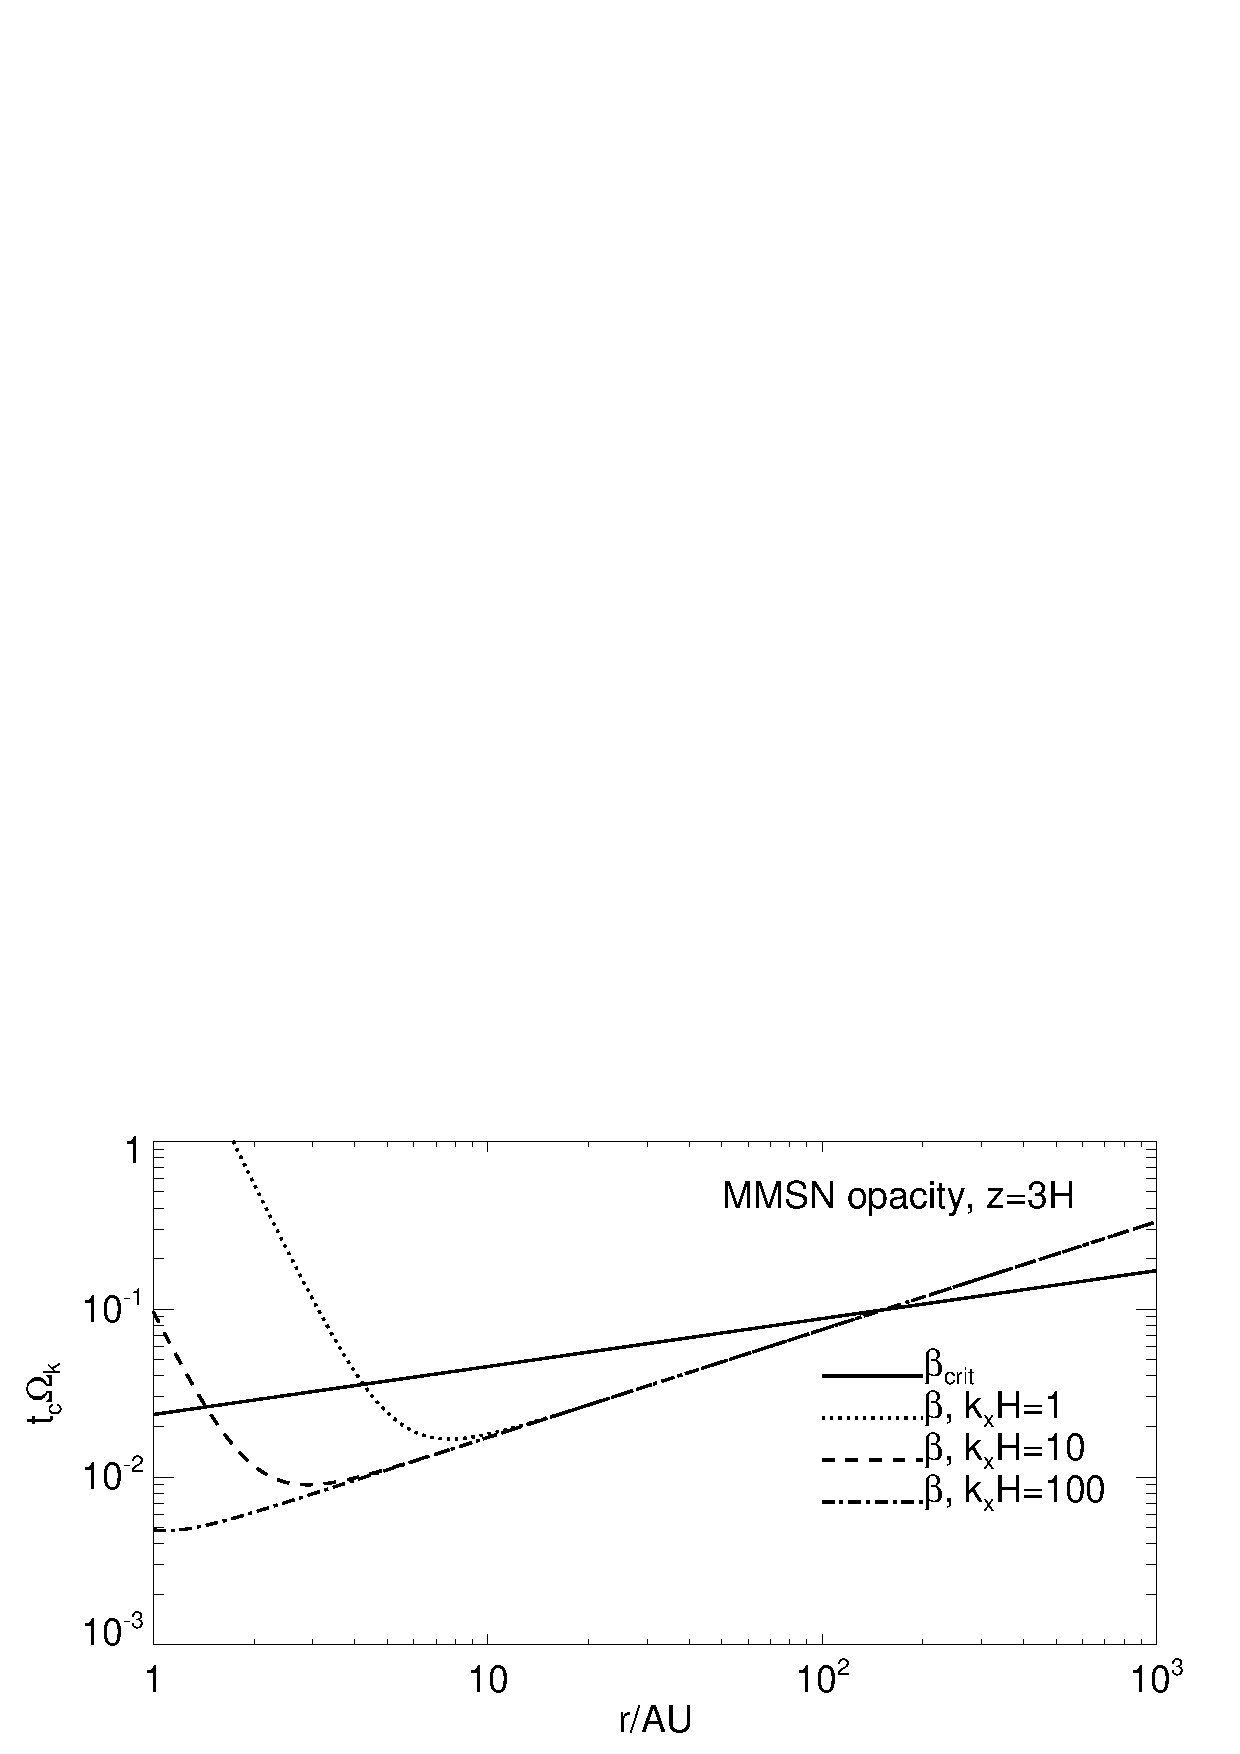
\includegraphics[scale=.47,clip=true,trim=2.5cm
  1.8cm 0cm 1cm]{figures/bcrit_mmsn_kap1_z3}\\
  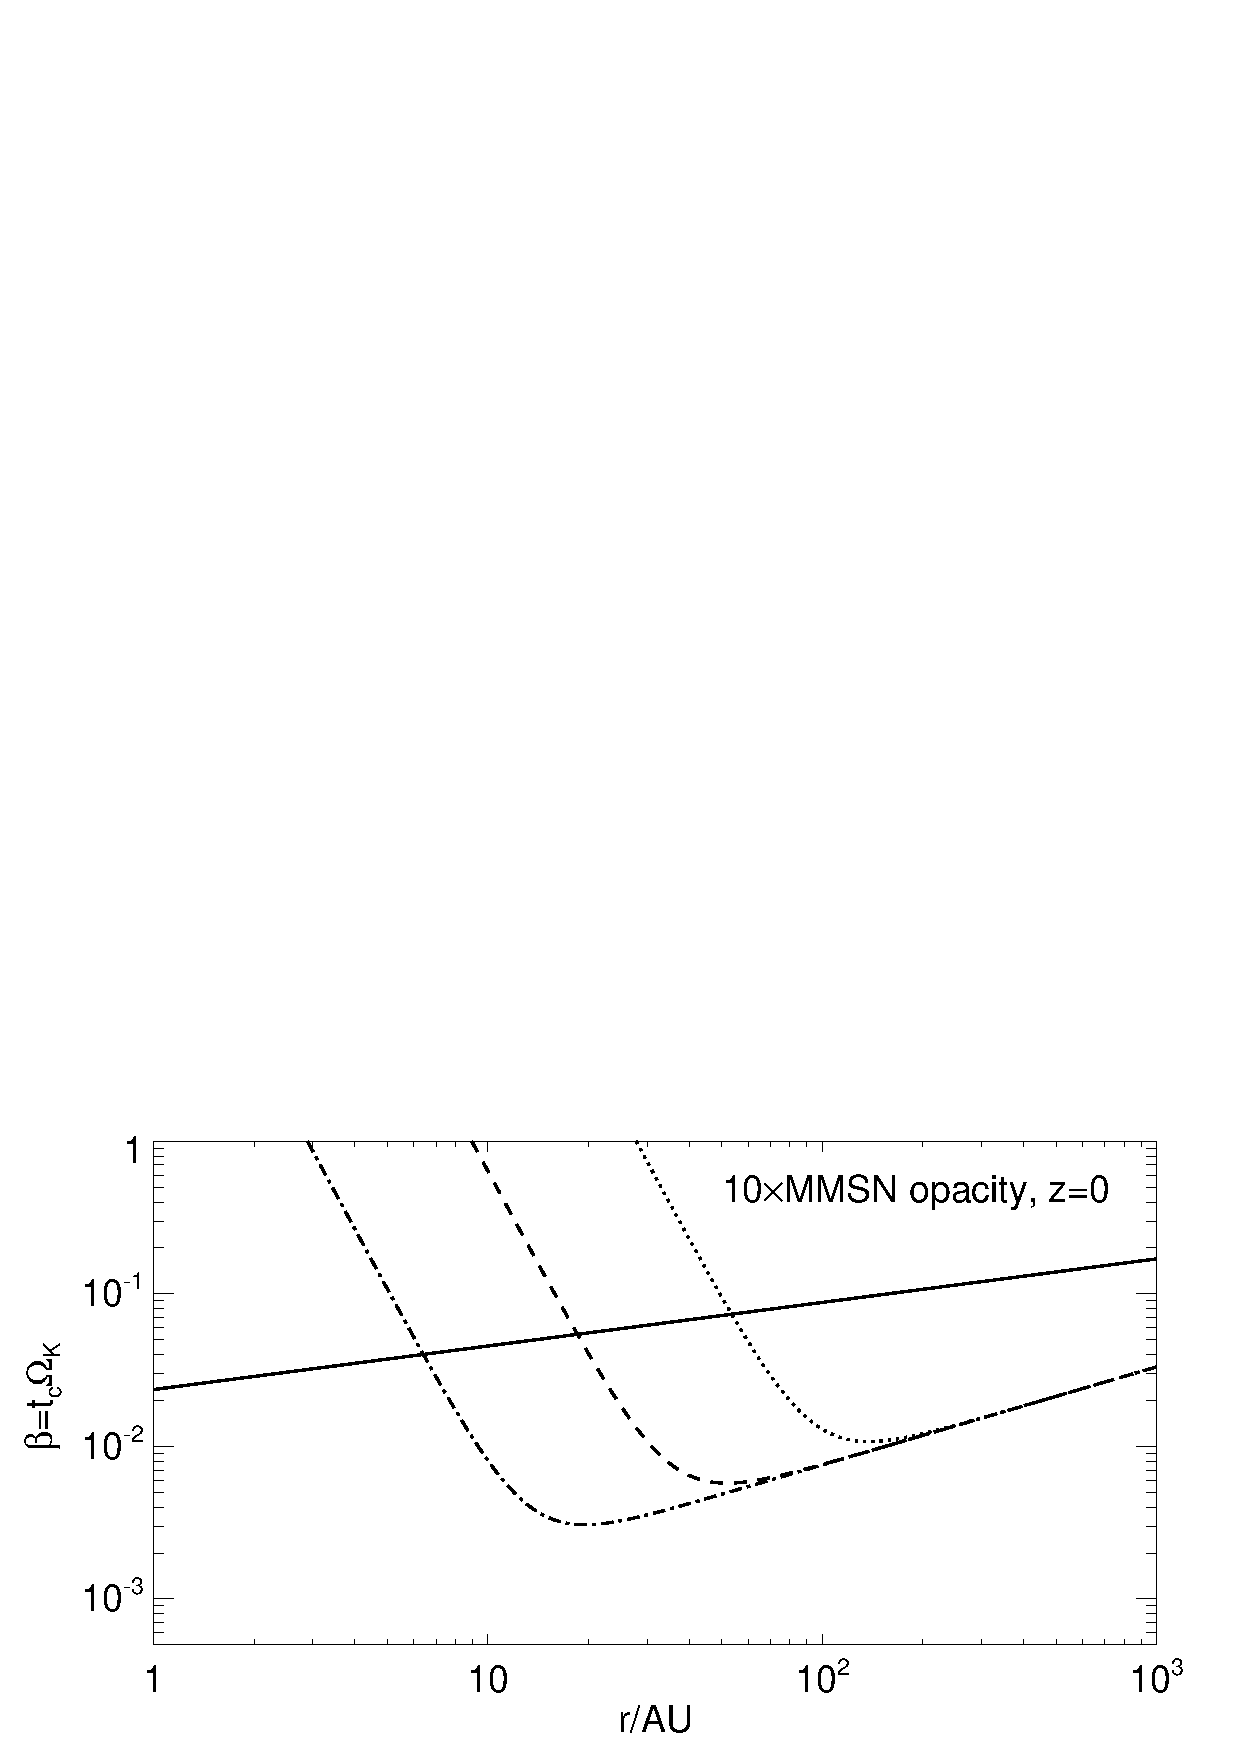
\includegraphics[scale=.47,clip=true,trim=0cm 0cm 0cm
  1cm]{figures/bcrit_mmsn_kap10_z0}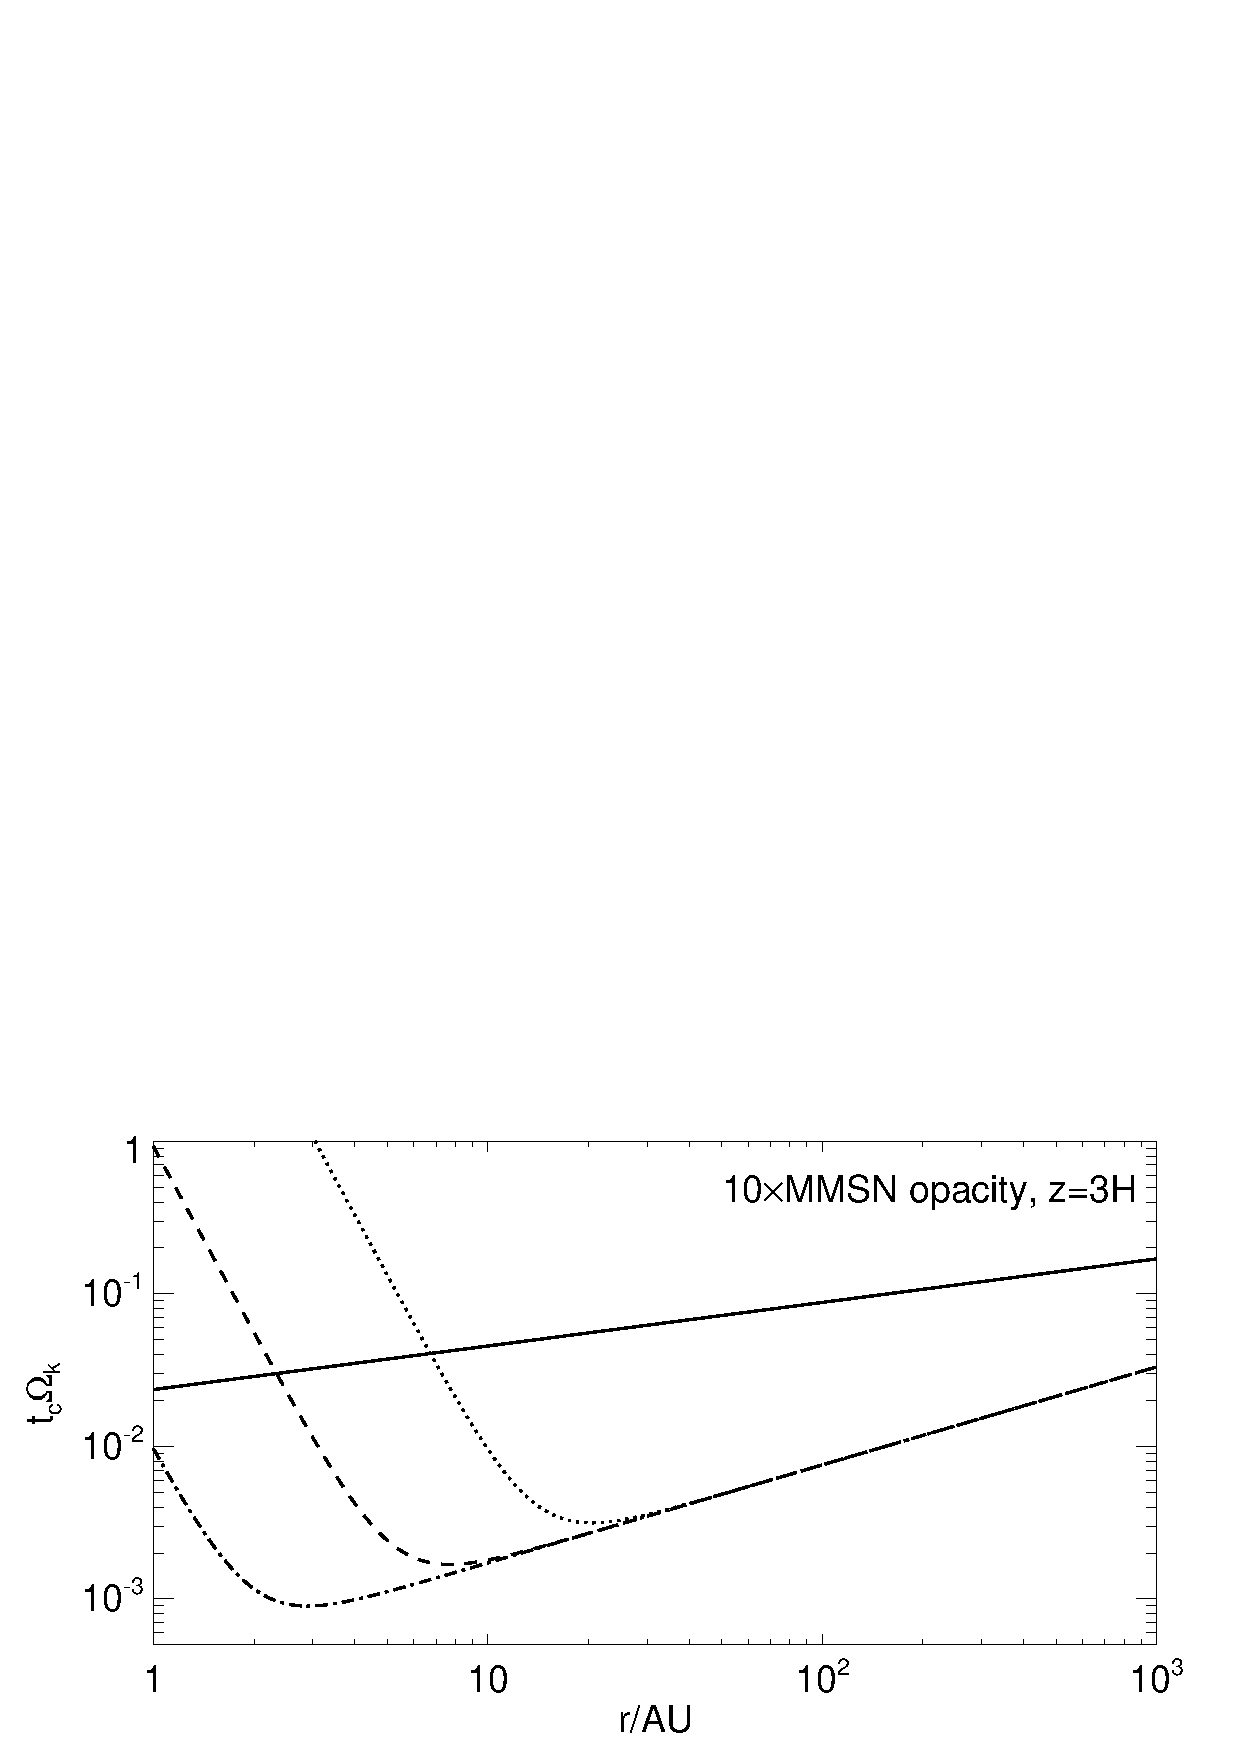
\includegraphics[scale=.47,clip=true,trim=2.5cm 0cm 0cm
  1cm]{figures/bcrit_mmsn_kap10_z3} 
  \caption{Dimensionless thermal relaxation timescales $\beta$,
    evaluated at the midplane (left) and at $z=3H$ (right) in the
    fiducial protoplanetary disk. Eq. \ref{beta_mmsn} is plotted  
    for three values of the 
    perturbation radial wavenumber: $\khat=1$ (dotted), $\khat=10$
    (dashed) and $\khat=100$ (dashed-dot), for three values of the
    opacity relative to the MMSN: $\hat{\kappa}_d=0.1$ (top),
    $\hat{\kappa}_d=1$ (middle) and $\hat{\kappa}_d=10$ (bottom).  
    The solid line is the 
    critical thermal relaxation timescale $\beta_\mathrm{crit}$.  
    % and 
    % $\beta<\beta_\mathrm{crit}$ is necessary for the fundamental isothermal VSI to operate  
    % for $\khat\gg1$. 
    \label{mmsn_bcrit_bcool}}   
\end{figure*}  

We remark that it is possible to satisfy $\beta < \beta_\mathrm{crit}$
for sufficiently large $\khat$. We
illustrate this in Fig. \ref{mmsn_bcrit_bcool_mink} by plotting at 
each radius the value of $\khat$ such  
that $\beta = \beta_\mathrm{crit}$. We thus expect that the VSI would only
occur on very small radial scales in the inner disk. % However, these
% may not be important as 
% our
% linear calculations suggest growth rates eventually decay for large
% $\khat$.  

However, disturbances with large $\khat$ may be subject to viscous
decay in a real disk. The viscous timescale for a perturbation lengthscale 
$l\sim 1/k_x$ is $t_\mathrm{visc} = 1/\alpha_s\khat^2\Omega $, where
$\alpha_s$ is the standard alpha viscosity parameter
\citep{shakura73}. Setting $t_\mathrm{visc}$ to be longer than the
minimum VSI growth timescale $1/\epsilon\Omega$ implies 
$\khat^2\lesssim \epsilon/\alpha_s$. Inserting $\epsilon \sim 0.05$,
we find only modes with $\khat\lesssim 20$ are relevant for
$\alpha_s\sim 10^{-4}$ or $\khat\lesssim 70$ for $\alpha_s\sim
10^{-5}$. \citep[These low viscosity levels are required for the
VSI, see][]{nelson13}.


\begin{figure}
  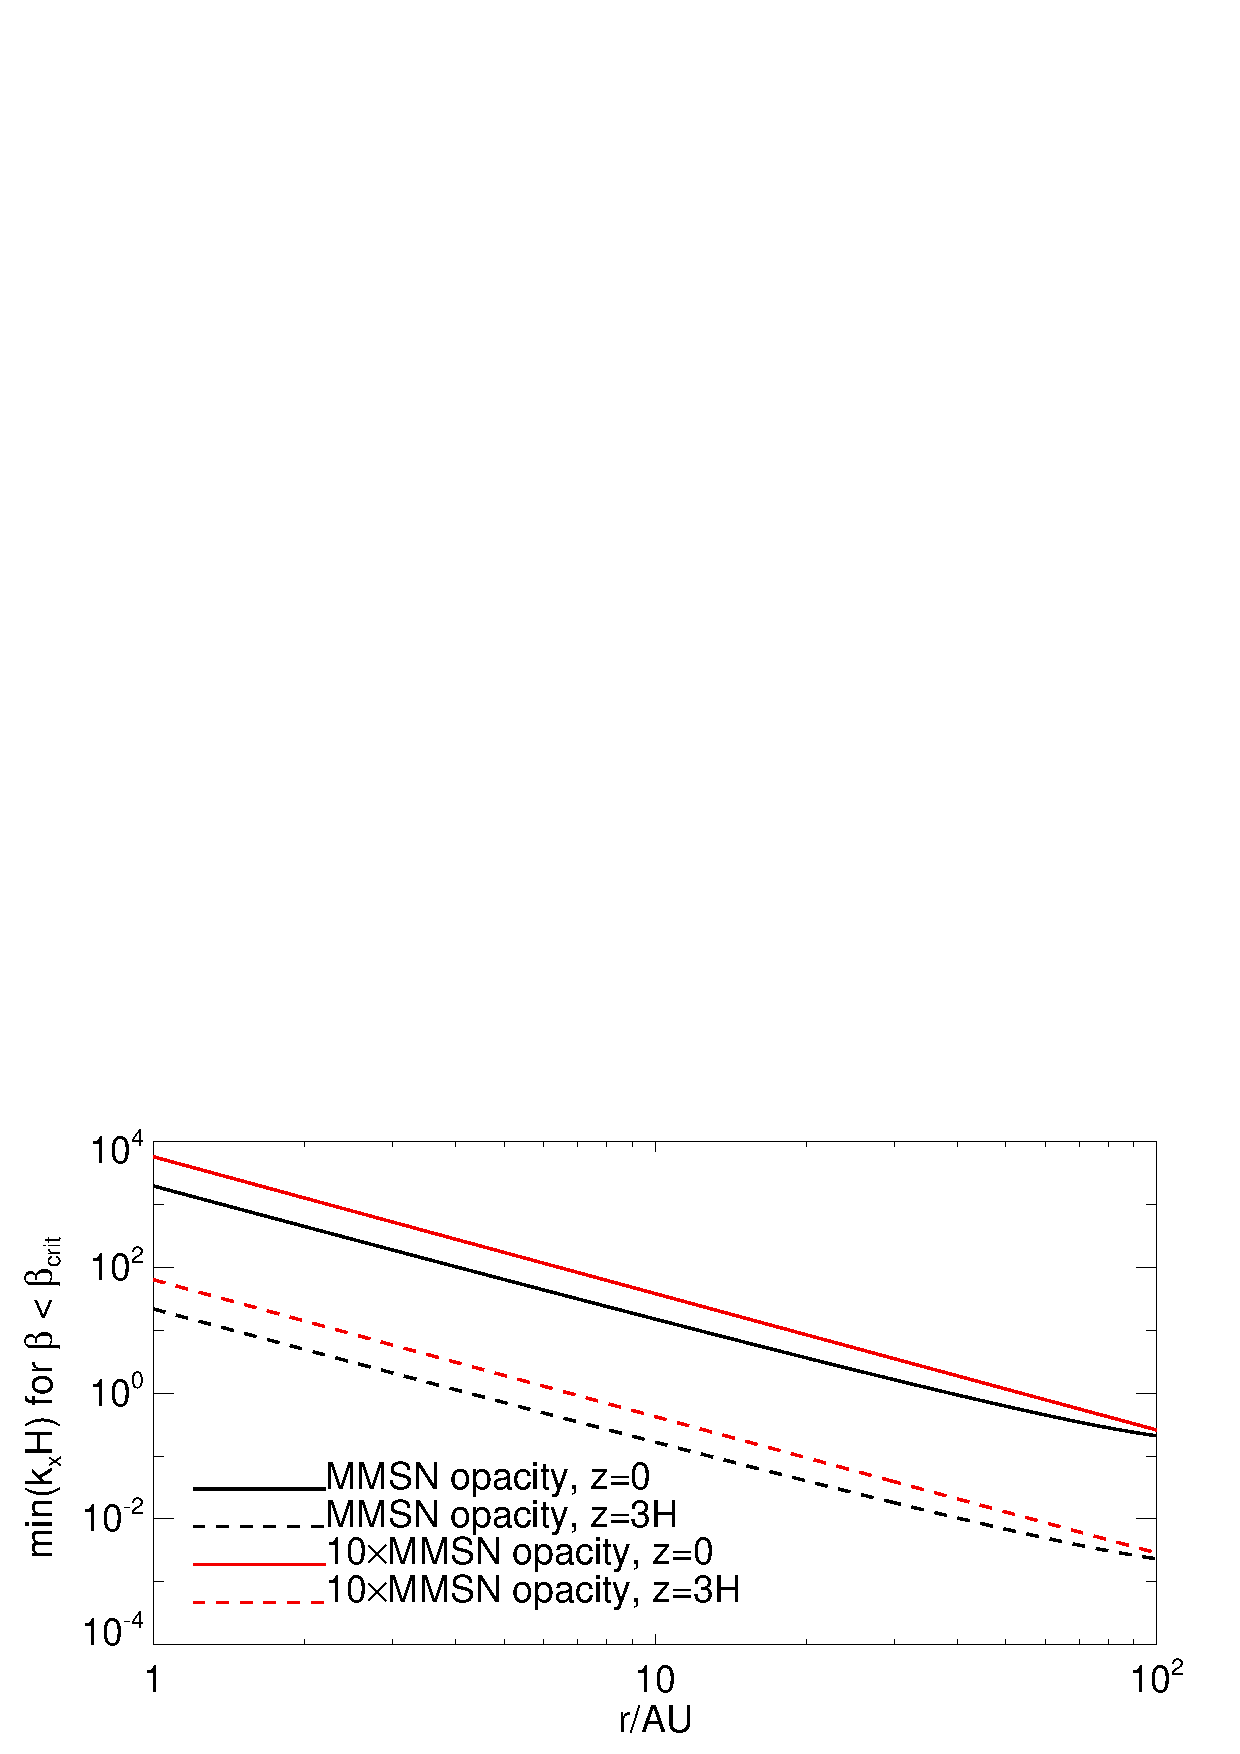
\includegraphics[width=\linewidth]{figures/bcrit_mink} 
  \caption{The minimum perturbation wavenumber $\khat$ in
    the MMSN such that the associated dimensionless thermal
    relaxation time  $\beta$ at $z=0$ (solid) and $z=3H$ (dashed) is
    less than the critical timescale $\beta_\mathrm{crit}$.   
    \label{mmsn_bcrit_bcool_mink}}   
\end{figure}  


\subsection{VSI in the MMSN}
Here we solve the linear stability problem in the MMSN with the scale and
height dependent thermal relaxation timescale defined by
Eq. \ref{beta_mmsn_simp}.  We use a vertical 
domain $z_\mathrm{max}=5H$. In Fig. \ref{mmsn_overall} we plot growth
timescales $t_\mathrm{grow} \equiv 1/\nu$ associated with the
fundamental mode in units of the local orbital time
$P_\mathrm{orb}\equiv 2\pi/\Omega_k$.    

In fact, we either only find the fundamental mode, or that it is the
most unstable, except for the appearence of some surface modes when considering large
$\khat\gtrsim 50$. However, surface modes are dependent on
boundary conditions and disturbances with large $\khat$ are more likely
subject to viscous decay, as discussed above. The dominance of the
fundamental mode is also observed in hydrodynamic
simulations of \cite{stoll14} which treat radiative cooling properly. 

% The dominance of the
% fundamental mode is consistent with our analytical discussion
% (\S\ref{iso_vsi_beta_crit}) and previous numerical results (\S\ref{therm_relax_eff}), which indicate  
% higher order modes are more easily stabilized by finite thermal
% relaxation.   

% In fact, for $\khat \lesssim 30$ we either only find the
% fundamental mode, or that it is the most unstable, and the associated
% growth rates are insensitive to $z_\mathrm{max}$. This is consistent with our
% analytical discussion (\S\ref{iso_vsi_beta_crit}) and previous
% numerical results (\S\ref{therm_relax_eff}), which indicate  
% higher order modes are more easily stabilized by finite thermal
% relaxation.   
% However, for large $\khat$ and/or $z_\mathrm{max}$, we also found
% surface modes with shorter growth times than those shown in
% Fig. \ref{mmsn_overall}. Such modes may not be robust because    
% they are affected by boundary conditions (\S\ref{surf_comment}) and/or
% viscosity in a real disk. 

We therefore consider Fig. \ref{mmsn_overall} as a representation of the
VSI in the MMSN. We see the VSI operates from $\sim 5$AU to $\sim
50$AU with growth timescales $\sim 30$---40 orbits. It is necessary to
consider smaller scales as $r$ decreases as the disk generally becomes
optically thick.  

Fig. \ref{mmsn_overall} is roughly consistent with the 
midplane thermal relaxation timescales for the MMSN ( 
Fig. \ref{mmsn_bcrit_bcool}, left middle panel). For example, for 
$\khat=10$ we find $\beta \gtrsim \beta_\mathrm{crit}$ for $r\lesssim
10$AU at $z=0$; and Fig. \ref{mmsn_overall} show stabilization inside
$\sim 8$AU where $t_\mathrm{grow}\to\infty$.  

\begin{figure}
  \includegraphics[width=\linewidth]{figures/eigen_compare_grow.ps}
  \caption{Characteristic growth times of the VSI in
    the MMSN. These are calculated using the scale and height
    dependent thermal relaxation given by Eq. \ref{beta_mmsn_simp}. 
    \label{mmsn_overall}}    
\end{figure}

\subsection{Numerical examples} 
We compare the VSI in the MMSN at $r=50$AU and $r=5$AU. We first show in
Fig. \ref{beta_compare}  the thermal timescale $\beta$ for a
perturbation wavenumber $\khat=30$. For comparison we also plot
$\beta_\mathrm{crit}$ at these radii. 

 \begin{figure}
  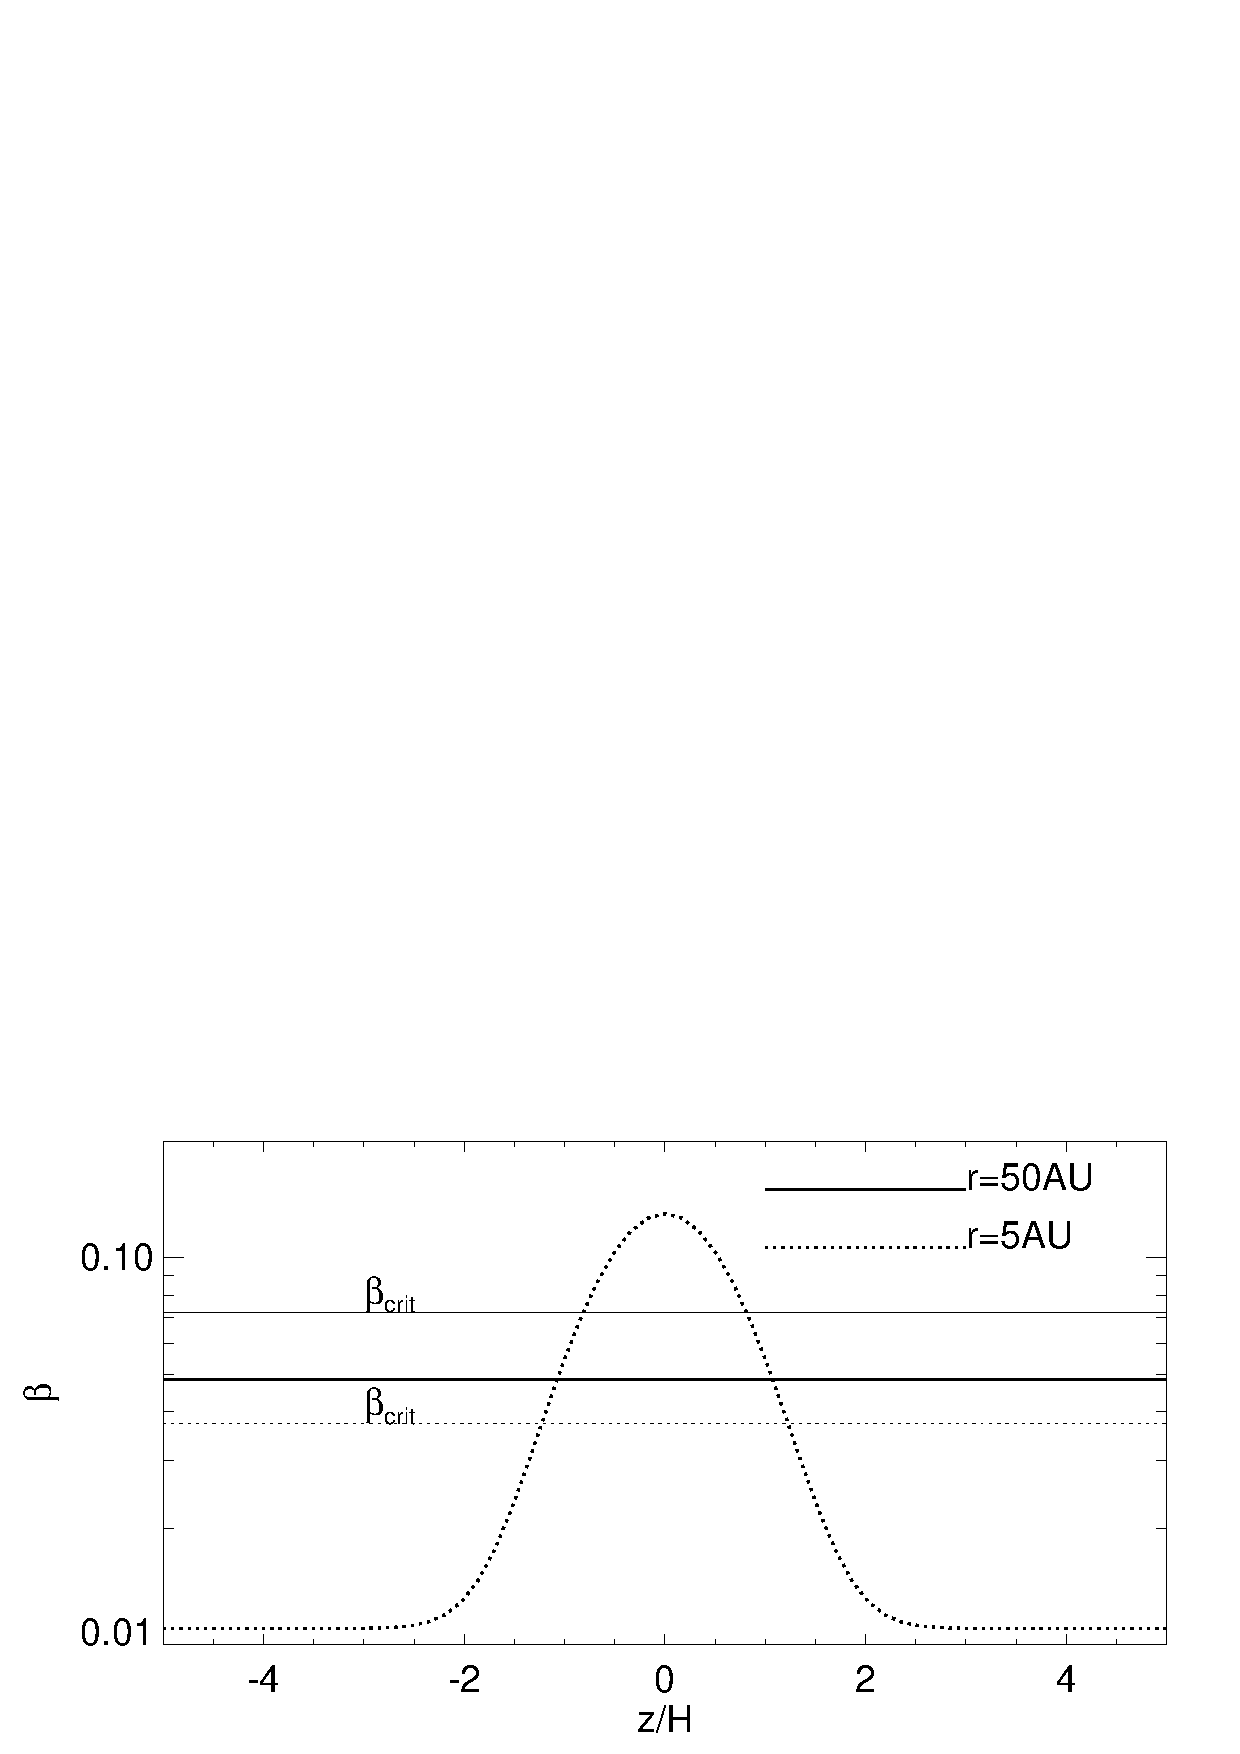
\includegraphics[width=\linewidth,clip=true,trim=0cm 0cm 0cm
  0cm]{figures/beta_compare}
  \caption{Thermal relaxation timescales in the MMSN at $r=50$AU
     and $r=5$AU for $\khat=30$ (solid lines). The
    corresponding thin horizontal dashed lines are the critical thermal
    relaxation timescales derived in linear theory. 
    \label{beta_compare}}
\end{figure}

The outer disk ($r=50$AU) is optically thin,
$\beta<\beta_\mathrm{crit}$  and  does not depend on height. 
Accordingly we expect, and find, the VSI 
operates at $r=50$AU. The inner disk ($r=5$AU) is optically
thick near the midplane and becomes optically thin away from it, such
that $\beta < \beta_\mathrm{crit}$ for $|z|\gtrsim1.25H$. In
fact, in this case  we also find the VSI to operate, but with much
reduced growth rates (when scaled by the local 
rotation). 

The corresponding vertical velocity perturbations are shown in 
Fig. \ref{mmsn_eigenvz}. Although at $r=5$AU $\beta$ depends on $z$,
the disturbance still occupies the fluid column due to the vertically
global nature of the fundamental mode. The fact that
we obtain the VSI despite $\beta > \beta_\mathrm{crit}$ near the
midplane suggests that the instability can operate 
provided $\beta < \beta_\mathrm{crit}$ for a sufficiently large
fraction of the vertical domain. However, the normalized growth times
are much longer at $r=5$AU than at $r=50$AU: %  for which  $\beta <
% \beta_\mathrm{crit}  \forall z$: 
$t_\mathrm{grow}\sim 40$ orbits at $r=50$AU, but $t_\mathrm{grow}\sim
400$ orbits at $r=5$AU. Thus, introducing an optically thick midplane
significantly reduces the efficiency of the VSI despite $\beta <
\beta_\mathrm{crit}$ away from the midplane.   

\begin{figure}
  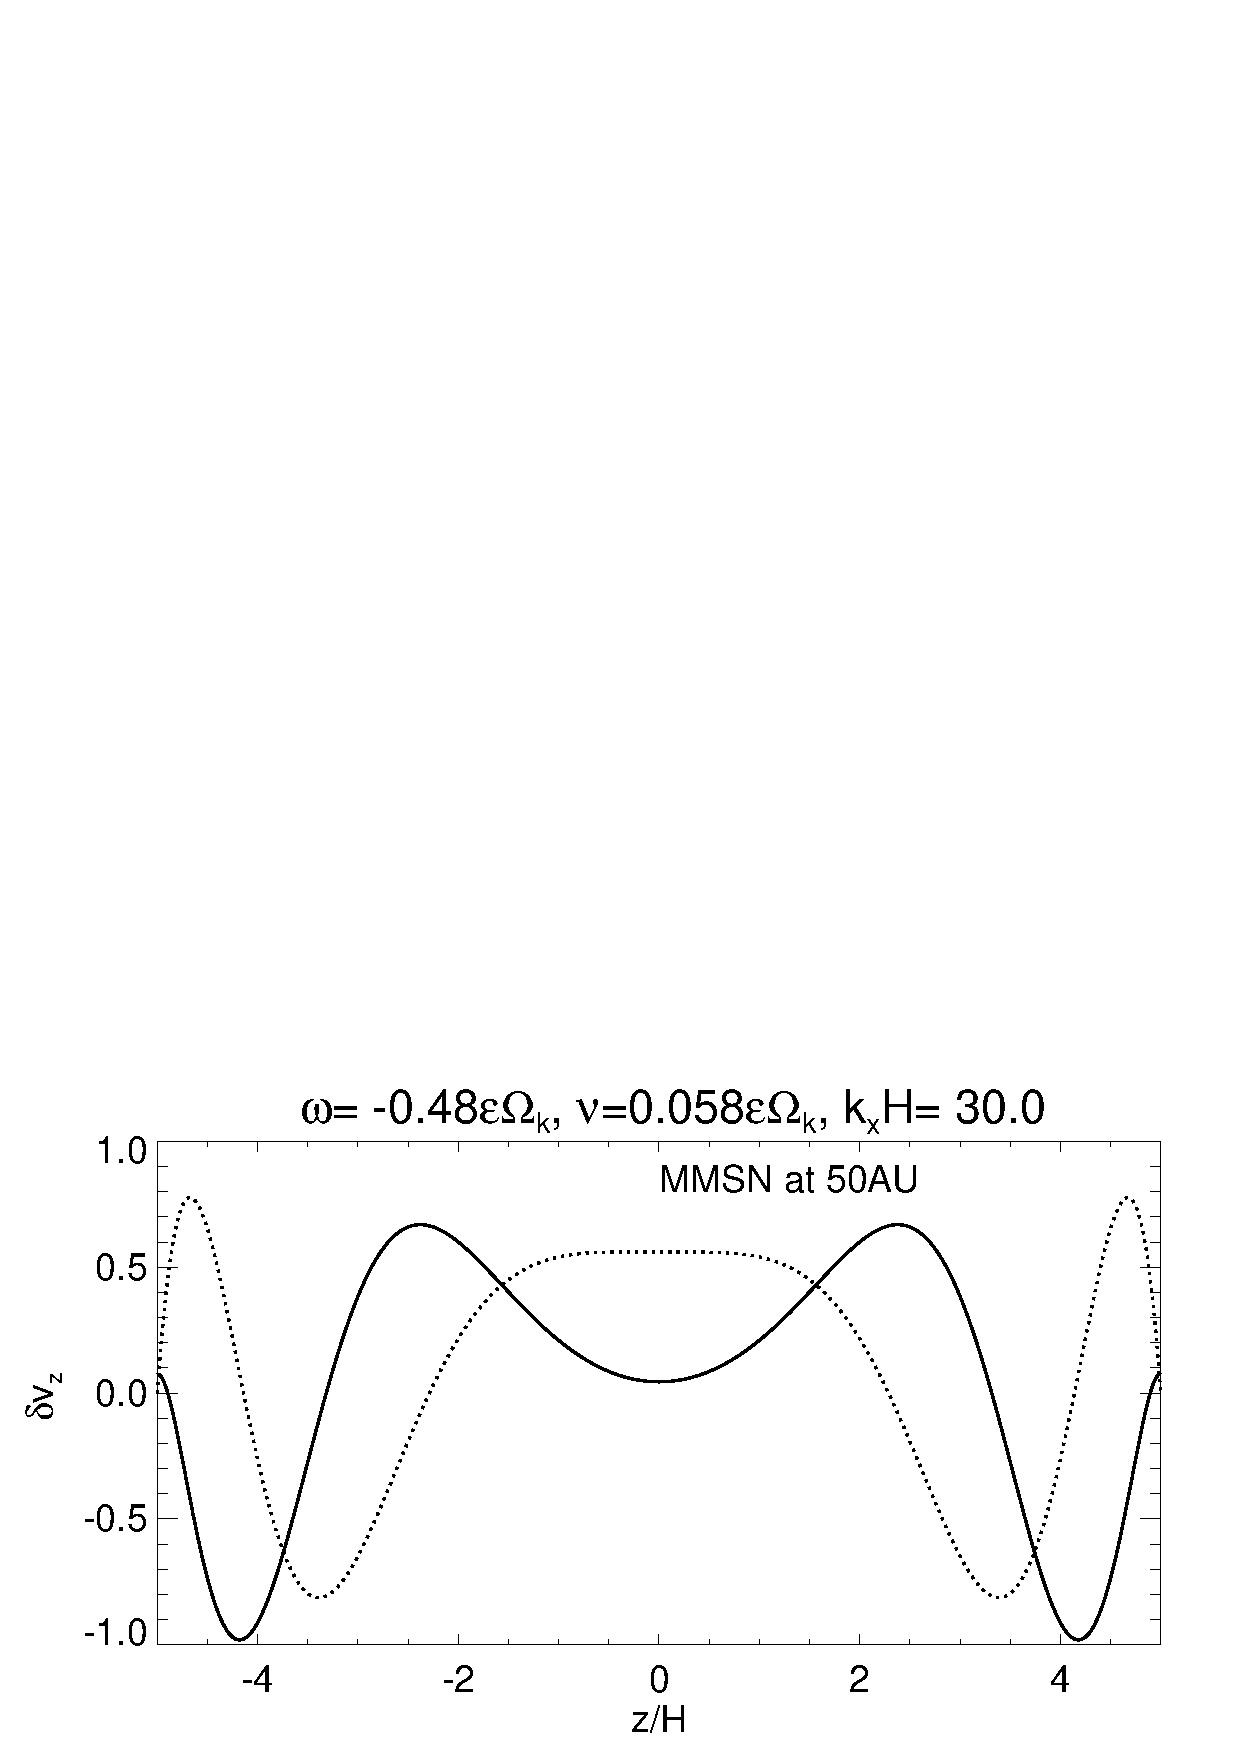
\includegraphics[width=\linewidth,clip=true,trim=0cm 1.75cm 0cm
  0cm]{figures/eigenvectorvz_mmsn_50AU}
  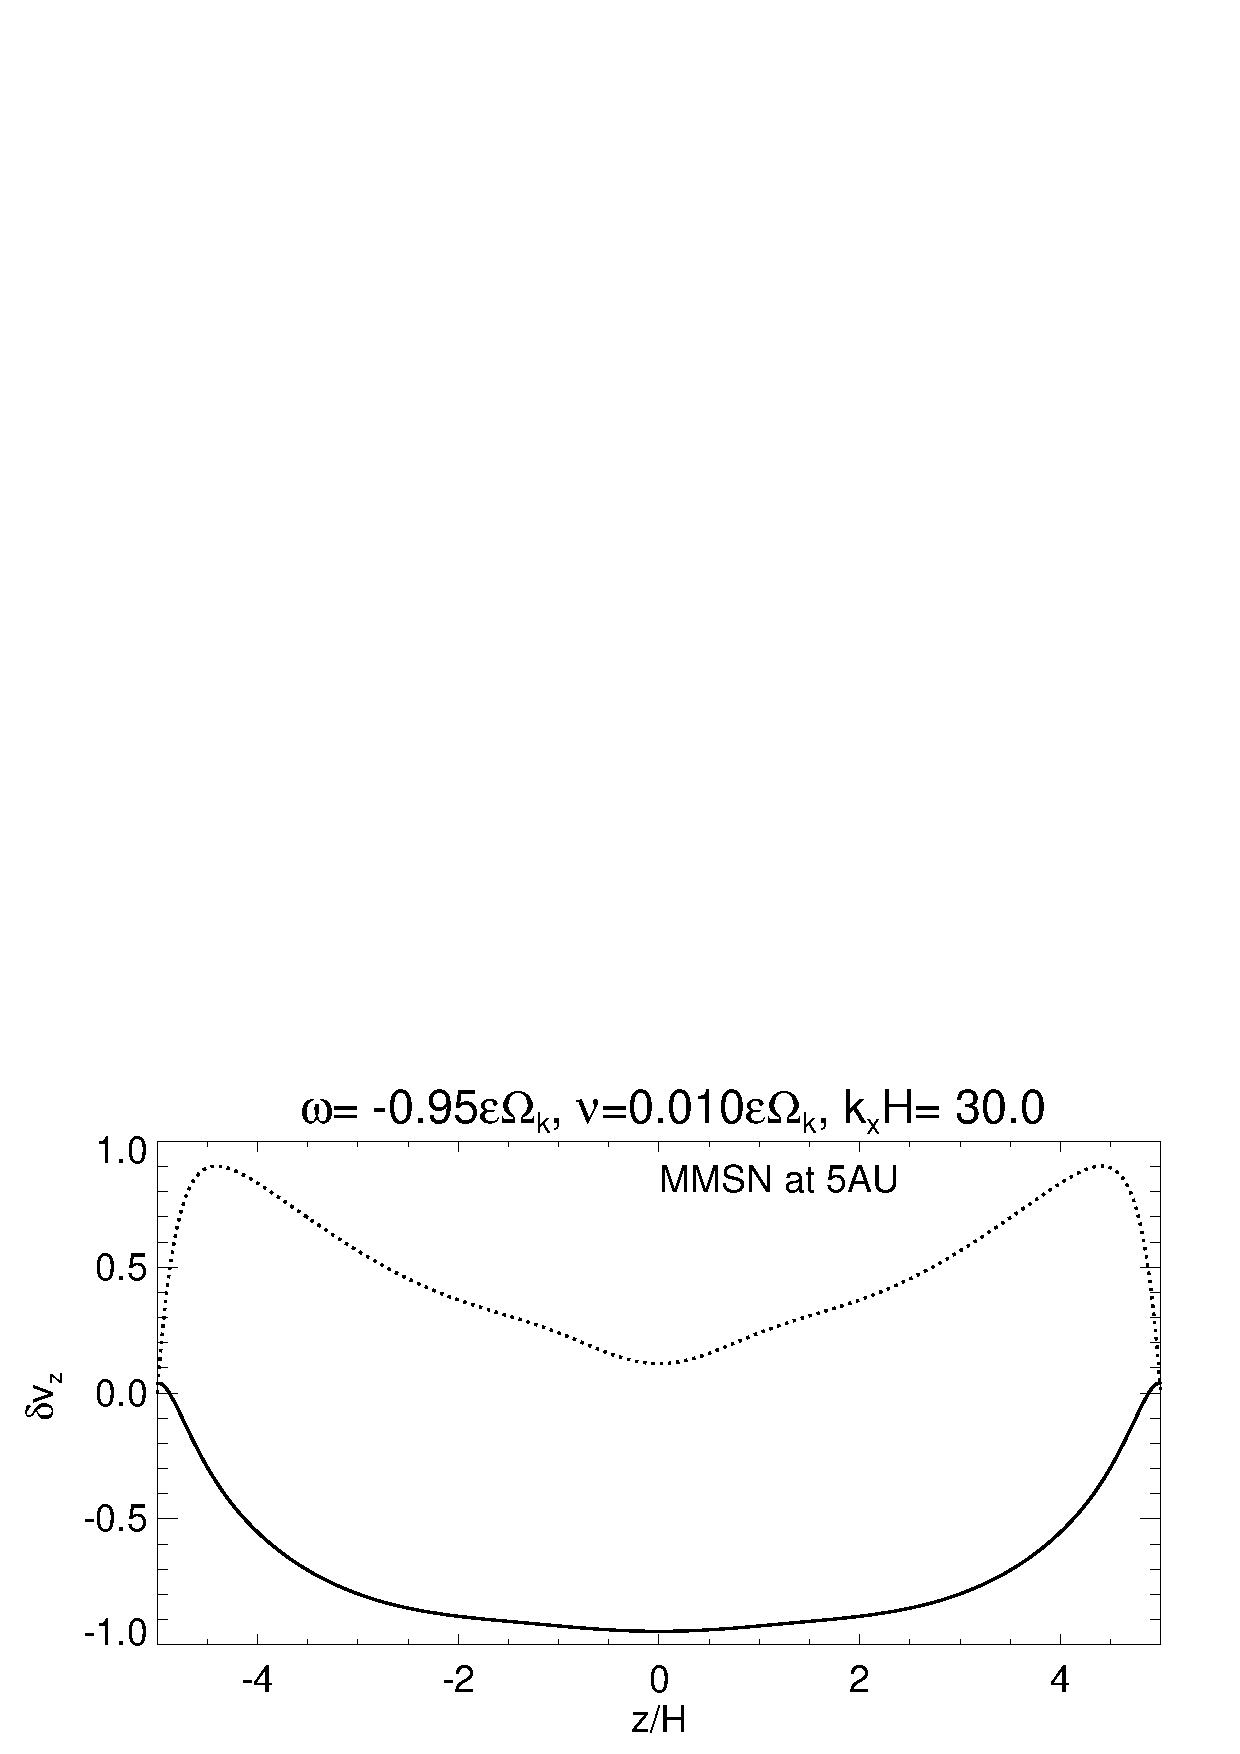
\includegraphics[width=\linewidth,clip=true,trim=0cm 0.0cm 0cm
  0cm]{figures/eigenvectorvz_mmsn_5AU}
  \caption{Vertical velocity perturbations of the VSI in the MMSN at 
    $r=50$AU (top) and $r=5$AU (bottom). The real (imaginary) part of 
    $\delta v_z$ is shown as
    the solid (dotted) curves. 
    \label{mmsn_eigenvz}}
\end{figure}
